\documentclass{article}

% Packages
\usepackage{titlesec}
\usepackage{graphicx}
\usepackage{hyperref}
\usepackage{amsmath}
\usepackage{listings}
\usepackage{float}
\usepackage{color}
\usepackage{caption}
\usepackage{subcaption}
\usepackage[sorting=none]{biblatex}
\usepackage{listings}

\addbibresource{references.bib}
\addbibresource{citations.bib}

\title{Implementation Of A Virtual Testbed For Secure IoT Firmware Update Using Blockchain}
\author{Tarun Chand}
\date{\today}

\begin{document}

\maketitle

\begin{abstract}
    With the increasing need and popularity of IoT devices and how integrated they are becoming in our daily lives and the industries, these devices make for a very lucrative target for malicious actors. And since these devices have such limited resources, the implementations for robust security features is a tradeoff to be made for the actual functionality the device was intended for. This makes them an easy target with high returns. This project aims at implementing a testbed for updating IoT device firmware using blockchain technology and offload the security features to the blockchain to make the process more secure while letting the device do what it was intended for.
\end{abstract}

\tableofcontents

\newpage

\section{Introduction}
\label{sec:introduction}
Introduction

The rapid gain in popularity of Internet of Things (IoT) devices has introduced new challenges, particularly in managing firmware updates securely and efficiently. Traditional methods often face issues related to trust, transparency, and decentralized control. In response to these challenges, this project presents an implementation of a testbed for an approach to IoT firmware updates leveraging blockchain and distributed storage technologies.
The motivation behind this project stems from the need for a robust and secure mechanism to manage firmware updates for IoT devices. The conventional centralized approaches pose vulnerabilities, such as single points of failure and susceptibility to malicious interference. By integrating blockchain technology and a distributed storage system, this project aims to address these concerns, ensuring the integrity, transparency, and security of the IoT firmware update process.
The primary objectives of this project are to establish a decentralized and secure framework for managing firmware updates in IoT devices. Key goals include:
\begin{enumerate}
    \item Immutable Record Keeping: Utilize blockchain technology to maintain an immutable ledger of firmware updates, preventing tampering and ensuring the integrity of the update history.
    
    \item Decentralized Storage: Employ the InterPlanetary File System (IPFS) for distributed and secure storage of firmware binaries, reducing the risk of data manipulation and enhancing the scalability of the system.
    
    \item Proof of Authority Consensus: Make use of a Proof of Authority (PoA) consensus mechanism to validate and authorize firmware updates, ensuring that only authorized parties can modify device firmware.
    
    \item Transparent and Secure End-User Updates: Provide a user-friendly interface for end-users to initiate firmware updates securely, with transparent verification mechanisms to guarantee the authenticity of the firmware being installed.
\end{enumerate}

\section{Related Work}
\label{sec:Related Work}

\subsection{Delivery}
There are various ways the update to firmware can be delivered to the IoT device. These methods include (but not limited to) \cite{nhtsa}:

\begin{itemize}
    \item eeprom burning: the firmware can be etched onto the eeprom of the device using specialized programmers. An example would be the ST-Link programmer for most ST-Microelectronics microcontrollers.
    \item wired pull: The device will ping the source of the update and check to see if there are any updates to be made. This could be automated or could be triggered by the user/owner and works well for devices that are constantly connected, for example home routers.
    \item wired push: The source of the update could push the updates onto the devices whenever they are ready.
    \item wireless pull: here, the device communicates over radio to ask for updates from its source.
    \item wireless push: the device can receive updates from the source wirelessly whenever the source is ready to send them.
\end{itemize}

Present challenges with delivery via the wireless methods according to \cite{blockchainupdate} are:

\begin{itemize}
    \item integrity of firmware while the update is performed
    \item centralized server infrastructure that can cause single points of failure
    \item low processing power and limited memory of IoT devices
    \item verifying the authenticity of firmware as a result of low processing power and memory of the devices
\end{itemize}

Networks with many nodes, like the ones seen in large scale sensor networks or home IoT devices, wireless methods for firmware upgrades are most suitable since connecting each device via cables and wires is not exactly scalable and convenient. But this method is the most vulnerable to attacks according to \cite{otaupdate}.

Authors of \cite{otaupdate} divide the stack of their implementation into hardware, protocol, proxy, blockchain, service, and application layers. This can be seen in figure on the next page:
\begin{figure}[H]
    \centering
    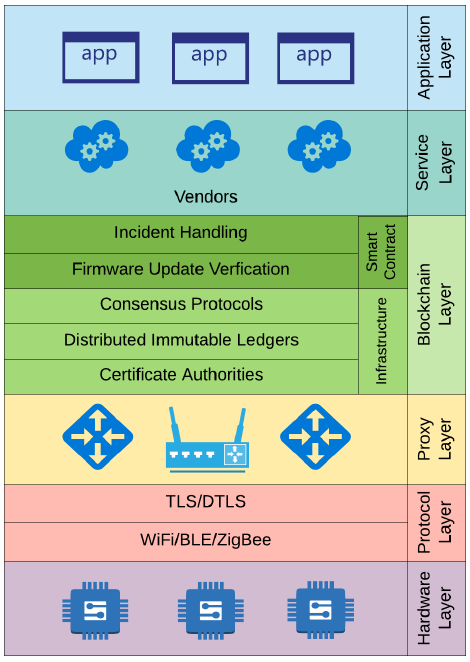
\includegraphics[width=0.5\textwidth]{ota01.png}
    \caption{Architecture of the OTA Update System.\cite{otaupdate}}
\end{figure}


The update mechanism their implementation looks the figure shown below:
\begin{figure}[H]
    \centering
    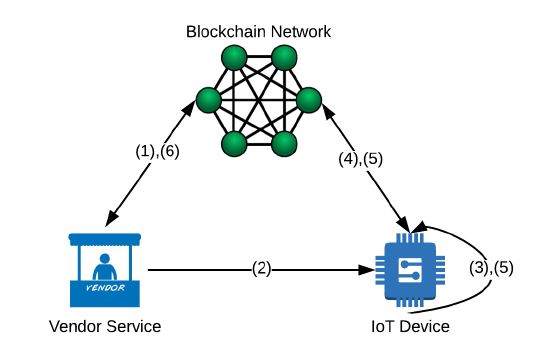
\includegraphics[width=0.7\textwidth]{ota02.png}
    \caption{OTA Update Process.\cite{otaupdate}}
\end{figure}


This is an example of a "wireless push" method where the vendor initiates a blockchain transaction for pushing the firmware onto the device when it is ready. The IoT device then queries the distributed ledger to verify if the update that is about to be performed was indeed pushed by the vendor. If this step fails, the update is aborted. There are various attributes the authors mention that are required for this process, which include transaction\_id, timestamp, deviceid, etc.

Another paper does something different with a concept the authors refer to as "genesis" node, smart contracts deployed by the genesis node, and a distributed storage to which the manufacturer uploads their firmware update \cite{blockchainupdate}:
\begin{figure}[H]
    \centering
    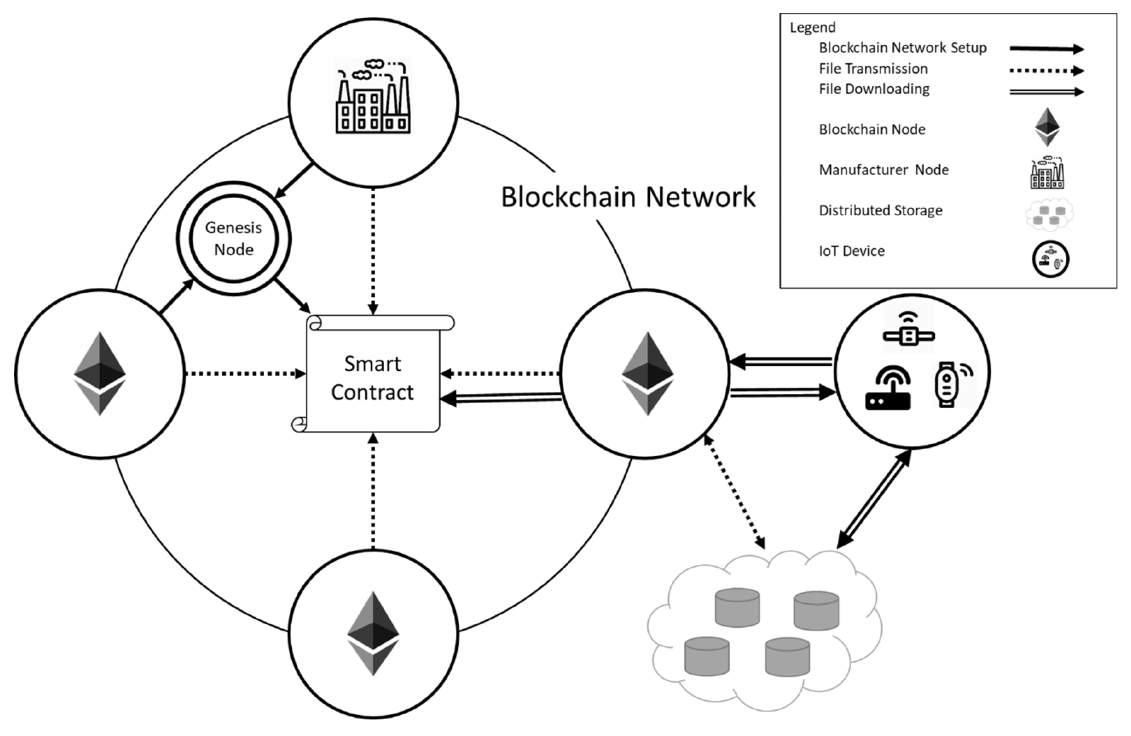
\includegraphics[width=0.7\textwidth]{blockchainupdate01.png}
    \caption{Blockchain-Based Firmware Update Process.\cite{blockchainupdate}}
\end{figure}


The firmware is first uploaded to a distributed storage like IPFS, and a unique identifier is generated for that file. The contents of the file are immutable and form a part of a blockchain. A smart contract is deployed by the genesis node, and the address of the smart contract is uploaded onto the IoT device. The process flow for their method looks like the figure below:
\begin{figure}[H]
    \centering
    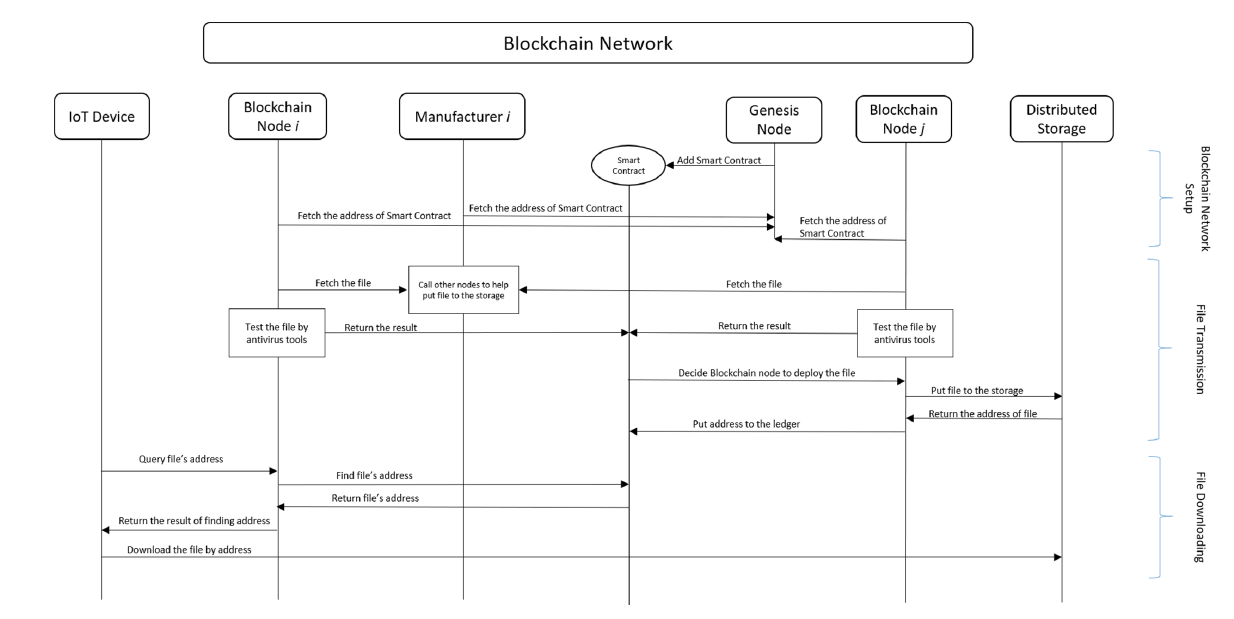
\includegraphics[width=\textwidth]{blockchainupdate02.png}
    \caption{Blockchain-Based Firmware Update Flow.\cite{blockchainupdate}}
\end{figure}

\subsection{Verification}
After the firmware is delivered to the end device, verification needs to be performed to check if the update was not modified by malicious actors, for example a man-in-the-middle attack. There are several challenges that we are faced with when it comes to verification of firmware on embedded devices according to \cite{verification}:

\begin{itemize}
    \item limited resources: the fundamental limitation for any embedded device has always been limited resources which prevent firmware developers from implementing anything other than the sole purpose the device was designed to do.
    \item lack of hardware trust: due to the previous point of limited resources, robust features are hard to implement on these devices.
    \item lack of memory separation: since programs on embedded devices run on bare metal, any kind of virtualization or abstraction is very difficult, which makes memory safety a difficult task.
    \item diversity: with so many kinds of microcontrollers with different instruction sets, it is hard to implement one robust method that can cover all these devices.
\end{itemize}

The authors of \cite{otaupdate} do have a verification process in place and is well integrated into their system since they are using blockchain to deliver their payload in the first place:
\begin{figure}[H]
    \centering
    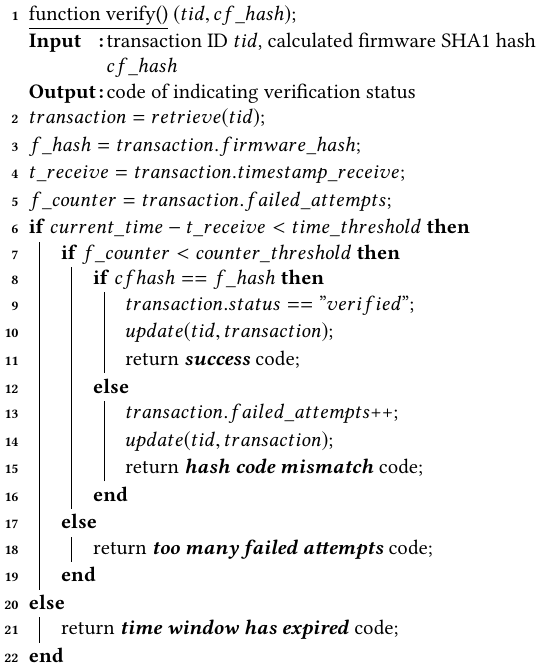
\includegraphics[width=0.7\textwidth]{ota04.png}
    \caption{Firmware Verification Process.\cite{otaupdate}}
\end{figure}


Another paper (\cite{verification}) proposes an architecture where there is a separate runtime that works like a pseudo-operating system to isolate the memory of the system and is responsible for the verification of the firmware installed on the device. The figure on the next page shows what the authors propose in the paper (solid borders show separate from the rest of the system):
\begin{figure}[H]
    \centering
    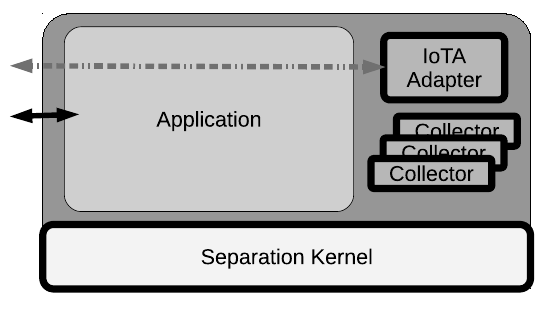
\includegraphics[width=0.7\textwidth]{verification01.png}
    \caption{Firmware Verification Architecture.\cite{verification}}
\end{figure}

However, a standalone paper that deals specifically with detecting anomalies in memory is worth taking a look. The authors use machine learning models to train and classify normal and compromised blob of firmware. The figure in the next page gives the overall architecture of the solution:
\begin{figure}[H]
    \centering
    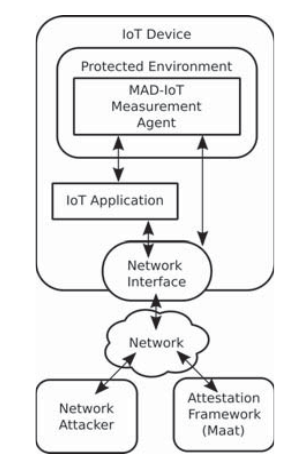
\includegraphics[width=0.7\textwidth]{mad01.png}
    \caption{Machine Learning-Based Anomaly Detection.\cite{mad}}
\end{figure}


There is a MAD-IoT measurement agent that periodically reads the firmware off of the device and runs the model to classify whether the firmware is compromised or is normally functioning. The authors test the model for metrics like accuracy, precision, recall, and F1 score and use both supervised and unsupervised learning methods. 

\subsection{Blockchain implementations}
Going through the papers and seeing the various frameworks of firmware upgrade using blockchain for verification, a number of models can be found. There is a choice for consensus model and what kind of network that can be used in order to implement such a system to deliver secure and authentic firmware to the end device.

The following are a few methods of consensus models used in blockchains available to us \cite{adoption}:

\begin{itemize}
    \item Proof of Work: In blockchain, proof of work requires participants to solve complex mathematical problems, demonstrating computational effort and securing the network.
    \item Proof of Stake: Unlike proof of work, proof of stake relies on participants' ownership or stake in a cryptocurrency to validate transactions and create new blocks in a more energy-efficient manner.
    \item Proof of Storage: Proof of storage involves participants providing evidence that they are storing a certain amount of data, ensuring network security and integrity through the commitment of storage resources.
    \item Proof of Authority: In a proof of authority consensus algorithm, validation is based on the reputation and authority of participants, often employed in private or consortium blockchains for enhanced governance.
    \item Proof of Elapsed Time: Developed by Intel, proof of elapsed time relies on a random lottery system where the participant with the shortest predetermined wait time is granted the right to create a new block, ensuring a fair and energy-efficient consensus mechanism.
\end{itemize}

The various structures of blockchain that are present can be listed out as follows \cite{adoption}:

\begin{itemize}
    \item peer to peer: Peer-to-peer networks facilitate direct communication and resource sharing between nodes, promoting decentralization and resilience in blockchain and distributed storage systems.
    \item sharding network: Sharding networks employ a partitioning technique to enhance scalability in blockchain, enabling the network to efficiently process and store data across multiple shards for improved performance.
    \item DAG network: Directed Acyclic Graph (DAG) networks, by structuring transactions in a non-linear fashion, enhance the efficiency of distributed storage and blockchain systems, allowing for parallel processing and faster consensus.
\end{itemize}

A detailed explanation of what the pros and cons of each model are can be found in \cite{adoption}, but the bottom line is, for an OEM making updates to an embedded device, proof of authority as a choice for consensus model makes the most sense with a peer to peer network where the firmware is uploaded onto a distributed storage and for anybody to verify.

\subsection{Frameworks}
The authors of \cite{otaupdate} have used an ESP8266 microcontroller that talks to a Wi-Fi router, a vendor service running at localhost, Hyperledger Fabric instance running and interacting with a node.js server, and Fabric Explorer as their UI frontend for their implementation. The interaction between the various modules of their work is shown below:
\begin{figure}[H]
    \centering
    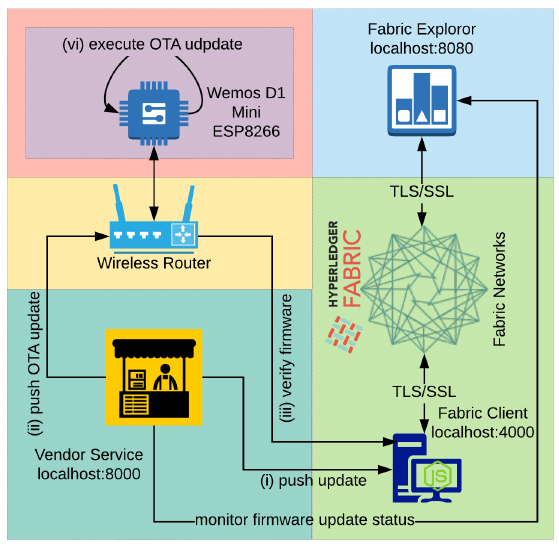
\includegraphics[width=0.7\textwidth]{ota03.png}
    \caption{Interaction Between Modules in OTA Update System.\cite{otaupdate}}
\end{figure}


Another implementation of a similar system is done by the authors of \cite{healthcare}. Their blockchain platform of choice was also Hyperledger Fabric, with Hyperledger Composer as their UI frontend. Although the authors mention that the development was done on a Linux environment, the actual execution takes place inside a Docker container, which is a very portable implementation and easy to replicate. They have a very specific use case of developing a system for healthcare, and their design reflects that. Following page has a class diagram of what they did for their implementation:
\begin{figure}[H]
    \centering
    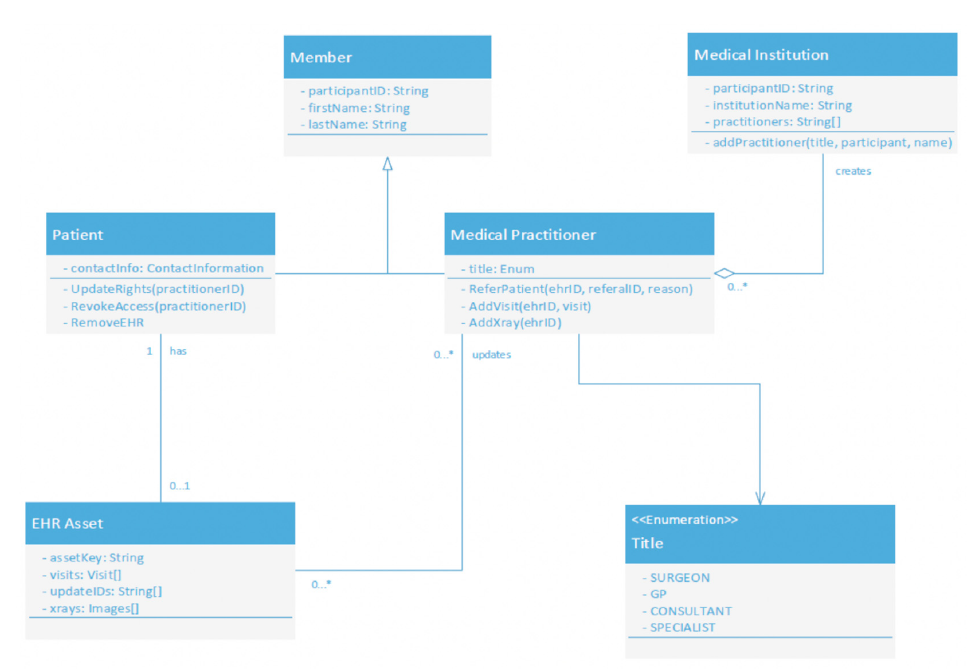
\includegraphics[width=\textwidth]{healthcare01.png}
    \caption{Class Diagram of Healthcare Implementation.\cite{healthcare}}
\end{figure}


The authors claim to have their results in compliance with the Europe's GDPR regulations.

\subsection{Summary}
From these works, it can be concluded that there are efforts being made to incorporate blockchain into the firmware update process for IoT devices and develop a trustless infrastructure for this process. And it is very much practical to do so as shown by the various implementations of the paper. The \cite{otaupdate} and \cite{lora} come close to creating a trustless system for update and verification wirelessly on a wide network, and \cite{healthcare} shows the implementation of a system with GDPR compliance using Hyperledger as its platform for blockchain implementation and the firmware being stored in a distributed storage as done by the authors of \cite{blockchainupdate}. In our testbed, elements of these different papers have been selected and adopted for implementation.

\section{Testbed Implementation}
\subsection{Definitions}

\subsubsection{Blockchain}
Blockchain is a distributed database that maintains a continuously growing list of records, called blocks, which are linked and secured using cryptographic signatures. It is a decentralized and distributed digital ledger that is replicated across a network of computers. Each block in the blockchain contains a collection of transactions, along with a cryptographic hash of the previous block in the chain. This creates an immutable chain of blocks, where any modification to a block would require changing all subsequent blocks in the chain.

The Ethereum whitepaper \cite{ethereumWhitepaper} describes blockchain as a state transition system described as the following function:
\[
\text{APPLY}(S,TX) \to S' \text{ or ERROR}
\]
for example: \(\text{APPLY}(\{ \text{Alice:} \$50, \text{Bob:} \$50 \}, \text{"send \$20 from Alice to Bob"}) = \{ \text{Alice:} \$30, \text{Bob:} \$70 \}\).

According to the Bitcoin whitepaper \cite{bitcoinWhitepaper}, when a new transaction is submitted to the network, it is broadcast to all nodes in the network. Each node validates the transaction and adds it to a pool of unconfirmed transactions. Miners, who are nodes that perform computational work to secure the network and validate transactions, do so in accordance with the consensus mechanism dictated by the particular blockchain protocol being used. The Ethereum blockchain, for example, uses proof of stake while the Bitcoin blockchain uses proof of work.

A transaction as illustrated in the Bitcoin whitepaper is shown in the figure in the next page:
\begin{figure}[H]
    \centering
    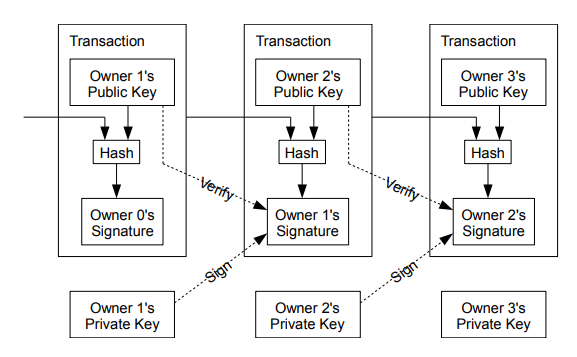
\includegraphics[width=\textwidth]{transaction_btcWp.png}
    \caption{Bitcoin Transaction.\cite{bitcoinWhitepaper}}
\end{figure}

Once the block is added to the chain, it is distributed to all nodes in the network, which validate the block's contents and cryptographic hash. If the block is valid, it is added to the local copy of the blockchain. Any nodes that do not agree with the block's contents can reject it and continue to validate transactions using the existing chain.

The use of cryptographic hashes, distributed consensus, and the consensus mechanism makes the blockchain highly resistant to tampering and hacking. This makes it a secure and transparent method for recording transactions and managing digital assets.

\subsubsection{Ethereum}
Ethereum is a decentralized, open-source blockchain platform that allows developers to build decentralized applications (dApps) and execute smart contracts. Here's how it works according to the Ethereum whitepaper \cite{ethereumWhitepaper}:

The state in the Ethereum blockchain is made up of objects called "accounts," with each account having a 20-byte address and state transitions being direct transfers of value and information between accounts. An Ethereum account contains four fields:
\begin{enumerate}
    \item The nonce, a counter used to make sure each transaction can only be processed once
    \item The account's current ether balance
    \item The account's contract code, if present
    \item The account's storage (empty by default)
\end{enumerate}

The term "transaction" is used in Ethereum to refer to the signed data package that stores a message to be sent from an externally owned account. Transactions contain:

\begin{itemize}
    \item The recipient of the message
    \item A signature identifying the sender
    \item The amount of ether to transfer from the sender to the recipient
    \item An optional data field
    \item A STARTGAS value, representing the maximum number of computational steps the transaction execution is allowed to take
    \item A GASPRICE value, representing the fee the sender pays per computational step
\end{itemize}

The state transition of the Ethereum blockchain according to the whitepaper \cite{ethereumWhitepaper} looks as follows:
\begin{figure}[H]
    \centering
    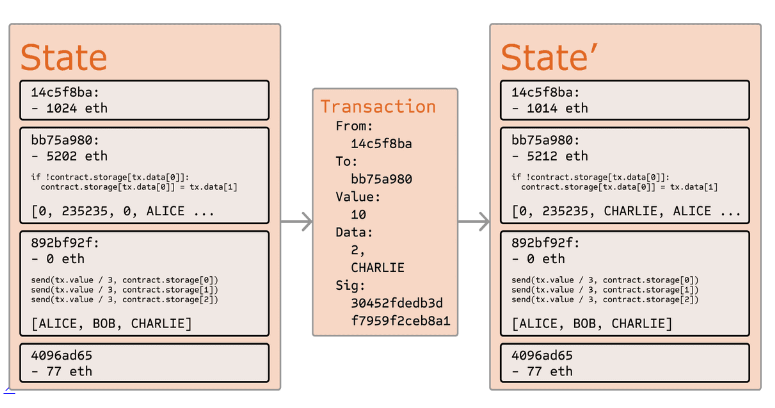
\includegraphics[width=\textwidth]{transition_ethWp.png}
    \caption{Ethereum State Transition.\cite{ethereumWhitepaper}}
\end{figure}

Ethereum uses a proof-of-stake consensus algorithm to secure its network, which relies on validators instead of miners.

At the heart of Ethereum are smart contracts, which are self-executing contracts that are stored on the blockchain. Smart contracts are written in a high-level programming language called Solidity, and they can be used to automate complex processes and transactions. Smart contracts can be triggered by specific events and can execute actions automatically without the need for intermediaries.

Ethereum also has its own cryptocurrency called Ether (ETH), which is used to pay for transactions on the network and incentivize validators. Ether can also be used to purchase and sell other digital assets, such as tokens that represent ownership in a dApp or a specific asset.

Ethereum's blockchain is composed of several key components:

\begin{itemize}
    \item Blocks: as mentioned earlier, Ethereum's blockchain is made up of a series of blocks that contain transactions and other data. Each block is linked to the previous block in the chain, creating an immutable and tamper-proof record of all transactions on the network.
    \item Gas: Ethereum uses a concept called "gas" to regulate the cost and complexity of executing smart contracts. Gas is a measure of computational work, and users must pay a fee in Ether to execute smart contracts on the network. The more complex the contract, the more gas it requires, and the higher the fee.
    \item EVM: The Ethereum Virtual Machine (EVM) is a runtime environment that executes smart contracts on the Ethereum network. The EVM is responsible for validating transactions, executing smart contract code, and storing data on the blockchain.
    \item Nodes: Ethereum is a decentralized network, which means that it is run by a network of nodes, rather than a single central authority. Nodes are computers that run the Ethereum software and validate transactions on the network.
\end{itemize}

\subsubsection{Geth}
Geth is one of the most popular clients for running a node on the Ethereum network. It is a command-line interface that enables users to interact with the Ethereum network, mine Ether, and execute smart contracts. Geth connects to the Ethereum network and downloads a copy of the blockchain. This copy of the blockchain is stored on the node running it, and it allows us to interact with the network.

In the words of Geth documentation \cite{gethDocumentation}, "Geth is an Ethereum execution client meaning it handles transactions, deployment, and execution of smart contracts and contains an embedded computer known as the Ethereum Virtual Machine."

Geth performs the following functions:

\begin{itemize}
    \item Interacting with the network
    \item Mining Ether
    \item Executing smart contracts
\end{itemize}

Geth can run in the following modes:

\begin{itemize}
    \item Full node: This mode downloads the entire Ethereum blockchain and validates all transactions. Running a full node allows you to have a complete copy of the blockchain, which can be useful for developing decentralized applications.
    \item Light node: This mode downloads only the header of each block and is much faster than running a full node. However, light nodes cannot validate transactions, so they rely on other nodes on the network to do so.
    \item Fast sync node: This mode downloads the entire blockchain, but it does so more quickly than a full node by skipping over certain details that are not necessary for validation.
\end{itemize}
The default behavior when geth is run is to start in Light node mode, which is what our project does as well.

\subsubsection{Geth Private Network}
Geth provides a number of tools and commands that allow for creation and managing of a private Ethereum network.

To create a private network, a genesis block needs to be setup, which is the first block in the new blockchain. The genesis block contains all of the initial configuration and settings for a new network, including the initial allocation of Ether, the network ID, and the consensus algorithm.

After this, Geth is used to initialize the new network and start mining blocks. Geth can also be used to add new nodes to the network, monitor the status of the network, and interact with smart contracts on the network.

To take part in the blockchain, each node needs to have an account represented by it's public address and a private key. When an account is created using geth, a password is needed to encrypt the private key and stored in a keystore, typically in the data directory along with the other blockchain data required for running a geth node. One thing to note is, this geth generated key pair is valid for any ethereum network including the mainnet and other popular test networks and not just our private network.

The implementation of proof of authority consensus mechanism is done when the geth clients are initialized and is handled by geth itself. There is a genesis.json file that every client has to be initialized before taking part in the blockchain network. The presence of "clique" field in the genesis file implies that we are using the proof of authority consensus mechanism and the following field with "extradata" field contains the list of accounts to be used as authoritative accounts that can mine new blocks. 

\subsubsection{Decentralized Storage}
Decentralized storage is a type of data storage system that does not rely on a central server or authority. Instead, it distributes data across a network of computers, making it more secure and reliable.

In a decentralized storage system, data is broken up into smaller pieces, encrypted, and then distributed across a network of nodes, which can be computers owned by individuals or organizations. Each node stores a small portion of the data, and no single node has access to the entire dataset.

When a user wants to retrieve the data, their client software contacts multiple nodes on the network and requests the pieces of data needed to reconstruct the original file. The nodes then transmit the requested data to the user's client, which decrypts the data and assembles it into the original file.

Since the data is distributed across multiple nodes, there is no single point of failure or attack. This makes it much more difficult for a hacker or malicious actor to compromise the data or tamper with it.

Another advantage of decentralized storage is its scalability. Since the data is distributed across multiple nodes, it can easily be scaled up or down to meet changing demand. This makes it an ideal storage solution for applications that require large amounts of data storage, such as storage of firmware for IoT devices.

There are several decentralized storage systems currently in use, including IPFS (InterPlanetary File System)\cite{ipfsWhitepaper}, Storj\cite{storj}, and Sia\cite{sia}.

\subsubsection{IPFS}
InterPlanetary File System is a decentralized file storage system that uses a distributed network of nodes to store and distribute files. Unlike traditional file storage systems that rely on centralized servers, IPFS allows files to be stored and accessed from multiple nodes.

The core concept behind IPFS is content addressing, which means that files are identified by a unique hash or fingerprint rather than by their location on a specific server. This allows files to be retrieved from any node on the IPFS network, rather than from a single server.

According to the IPFS whitepaper \cite{ipfsWhitepaper}, this is what the life cycle of data looks like:

\begin{enumerate}
    \item Content-addressable representation: this includes chunking the file and hashing each chunk.
    \item Pinning: this involves advertising and providing the data a node has.
    \item Retrieval: this involves content routing, block fetching from the Merkle DAG, and verification.
    \item Deleting: this is always a local operation for a node.
\end{enumerate}

Here's how IPFS works:

\begin{itemize}
    \item Add content: To add content to the IPFS network, we first create a file or folder on your local computer. You then use IPFS client software to add the content to the network, which generates a unique hash that identifies the content.
    \item Distribute content: The IPFS network is made up of a distributed network of nodes, which can be computers owned by individuals or organizations. When we add content to the IPFS network, the content is automatically distributed across multiple nodes.
    \item Retrieve content: To retrieve content from the IPFS network, we use the unique hash generated when the content was added. The client software then searches the IPFS network for nodes that have a copy of the content and retrieves the pieces needed to reconstruct the original file.
    \item Update content: If we need to update a file that has already been added to the IPFS network, we need to create a new version of the file, add it to the network, and calculate the new hash for the file. We then have to change the address in the smart contract with this new hash. It is difficult to make changes and update existing content once it has been added since data on the IPFS network is immutable.
\end{itemize}

\subsubsection{IPFS Private Network}
It is possible to host a private IPFS network. One of the key benefits of IPFS is that it is designed to be easily deployable and customizable, allowing individuals and organizations to set up their own IPFS nodes and networks.

To host a private IPFS network, these general steps need to be taken:

\begin{itemize}
    \item Install and Configure IPFS: This involves setting up storage and networking parameters, as well as configuring access control and security settings. The important one being generation of a swarm key which can be used by other nodes to join the network which we can refer to as a swarm.
    \item Add content: Once the IPFS node is up and running, we can add content to the network by using IPFS client software to create and upload files or folders. This will generate a unique hash that identifies the content on the IPFS network.
    \item Distribute content: The distribution of the content is done by the ipfs clients present in the same swarm. The uploaded file propagates through the network ready to be retreived by referencing the content id of the file.
    \item Retrieve content: To retrieve content from the private IPFS network, we can use IPFS client to search for the content by its unique hash.
\end{itemize}

Hosting a private IPFS network can cause the following problems:

\begin{itemize}
    \item storage requirements: If the data being stored in the IPFS network exceeds the storage available in the client devices, this can pose as a problem since each IPFS client also acts as storage and there are redundant copies of the same file in multiple locations. This is one downside of having a distributed storage solution.
    \item NAT: IPFS nodes do not behave well with devices behind NAT. There are solutions like UDP punchthrough, use of WebRTC or NAT traversal for this problem. For our implementation, there is a port forwarding in place to get around the problem and the ports responsible for communication with other nodes in the swarm (port 4001) is exposed through the NAT.
\end{itemize}

\subsection{Design}
The following block diagram shows the overall architecture of the system used in this project:

\begin{figure}[H]
    \centering
    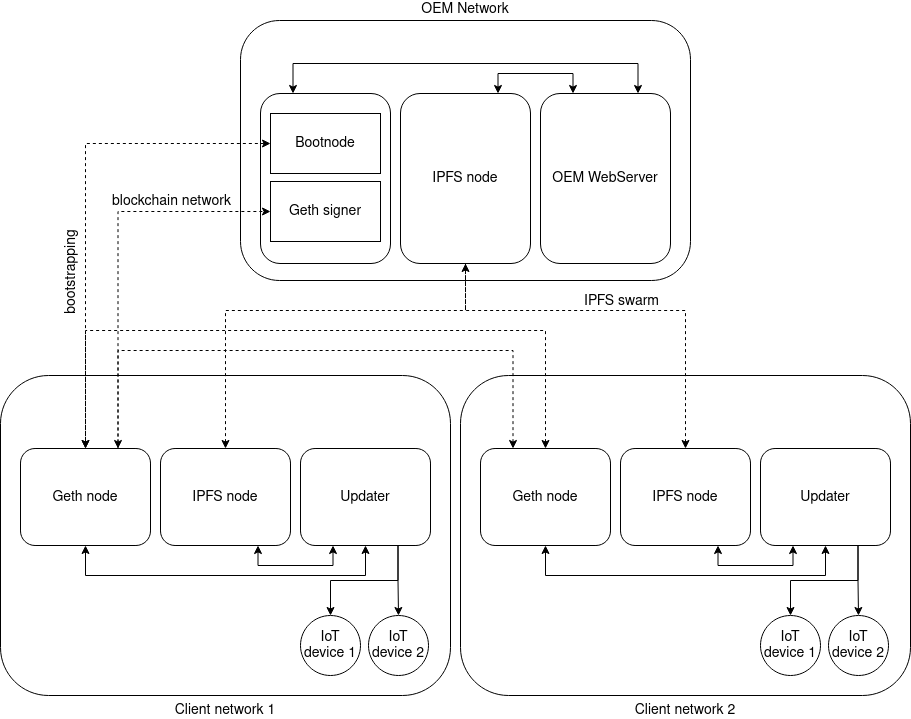
\includegraphics[width=\textwidth]{architecture.png}
    \caption{Architecture}
\end{figure}


The figure examines the high-level architecture of the system, including the major components, interactions, and data flows.

The IoT device firmware upgrade process using blockchain and distributed storage involves several components working together seamlessly. At the heart of the OEM network are two main servers - a web server and a Geth signer server. The web server is responsible for handling requests from various users, such as OEM manufacturers and end-users, while the Geth signer server provides the necessary infrastructure for securely storing and retrieving firmware update metadata on the blockchain.

When an OEM manufacturer wants to release a new firmware version for their devices, they use the web server to upload the updated firmware. This firmware is then stored on a distributed storage system, specifically InterPlanetary File System (IPFS), which is also running on the same server as the web server. The IPFS system assigns a unique Content ID (CID) to the firmware, which acts as its digital fingerprint. This CID is then passed on to the Geth signer server, where it is used to create a new transaction on the blockchain.

The Geth signer is responsible for ensuring that only authorized parties can update the firmware on the devices. The authorized party being the OEM manufacturer that is in posession of the private key for the account mentioned in the genesis.json file. Only those accounts mentioned in the genesis.json are able to mine new blocks. 

One of the key reasons IPFS is chosen instead of storing the firmware binaries directly on the blockchain is that IPFS is better suited for storing larger files. Storing large files directly on the blockchain can lead to bloat and increased storage costs. Geth is not particularly optimized to sync large blocks across the blockchain network and hence not a good choice to store large blobs of data directly on the chain. By using IPFS, we can keep the blockchain lean and focused on storing metadata, while still providing a secure and decentralized storage solution for the firmware blobs themselves.

On the other side of the system, there is a second web server that runs on the end-user's updater device. This web server provides a user interface for the end-user to initiate firmware updates on their device. When the end-user requests an update, the web server communicates with the local Geth node (which is not a signer) to retrieve the latest firmware version from the IPFS node. The web server downloads the firmware from the IPFS node and applies the update to the IoT device.

\subsection{Data Flow}
Moving onto the data flow of this project, following is a high-level overview of how data will flow through the system:
\begin{itemize}
    \item The manufacturer releases a new firmware version for a device.
    \item The manufacturer uploads the firmware binary to IPFS and gets a CID that represents the firmware in return
    \item The manufacturer records the CID of the file in the blockchain with the help of the deployed smart contract.
    \item An end-user initiates a firmware update on their device.
    \item The client's updater device contacts the blockchain to retrieve the content id of the latest firmware for a given device
    \item The updater device downloads the firmware binary from IPFS using the CID recorded in the smart contract.
    \item The updater device installs the firmware update onto the IoT device in the local network.
\end{itemize}

The following sequence diagram represents the overall data flow of this project:
\begin{figure}[H]
    \centering
    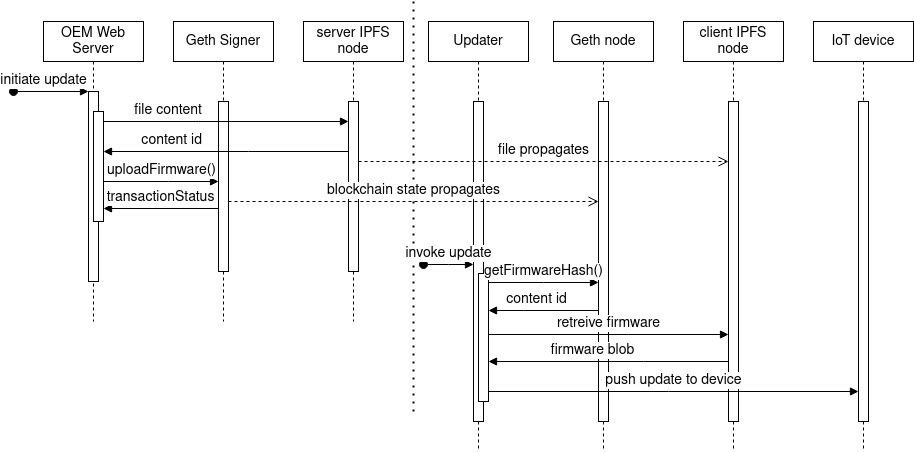
\includegraphics[width=\textwidth]{sequenceDiagram.png}
    \caption{sequence Diagram}
\end{figure}

\subsection{Pseudocode}
In order to provide a clear and structured understanding of the IoT device firmware upgrade system's inner workings, the following section on pseudocode is presented:
Let's take a look at the pseudocode for each component, beginning with the OEM server's firmware upload process.

\begin{lstlisting}
    
    # Function to Upload Firmware
    function Upload(firmwareFile, deviceName):
        connect_to_ethereum()  # Connect to the Ethereum node
        get_account()  # Get the Ethereum account address
        get_contract_abi()  # Fetch the contract ABI
        get_contract_address()  # Fetch the contract address
        connect_to_ipfs()  # Connect to the local IPFS node
    
        # Upload the firmware:
        ipfs_hash = upload_firmware_to_ipfs(firmwareFile)
        record_transaction_on_blockchain(ipfs_hash, deviceName)
        return {'status': transaction_status, 'hash': ipfs_hash}
\end{lstlisting}

Note that proof of authority mechanism is being handled by the geth signer node and is configured using the genesis.json file when the blockchain is initialized.

And the following is how the end users' device would apply the firmware update from the web UI.

\begin{lstlisting}
    # Function to Fetch Latest Firmware
    function Update(device):
        connect_to_ethereum()  # Connect to the Ethereum node
        get_contract_abi()  # Fetch the contract ABI
        get_contract_address()  # Fetch the contract address

        latest_firmware_hash = fetch_latest_firmware_hash_from_blockchain(device)
        firmware_data = fetch_firmware_data_from_ipfs(latest_firmware_hash)

        apply_firmware_update(firmware_data)
\end{lstlisting}

As for the smart contract, the smart contract does the basic function of storing the latest firmware hash for each device and providing an interface for outside to store and retreive those hashes.
\begin{lstlisting}
contract FirmwareUpdate {

    mapping(string => string) deviceToFirmwareMapping;

    function getLatestFirmwareHash(string device) view returns (string) {
        return deviceToFirmwareMapping[device];
    }
    
    function storeFirmware(string ipfsHash, string device) public payable {
        deviceToFirmwareMapping[device] = ipfsHash;
    }

}

\end{lstlisting}
\newpage
\subsection{Development}
The following figure summarizes how the project has been structured and implemented:
\begin{figure}[H]
    \centering
    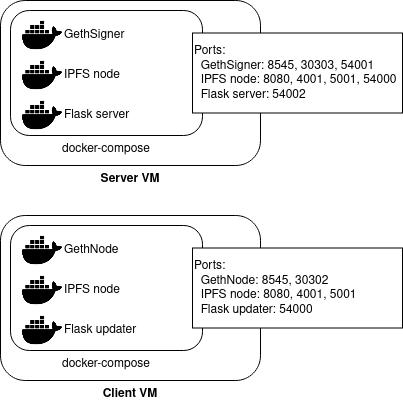
\includegraphics[width=0.8\textwidth]{development.png}
    \caption{Project structure}
\end{figure}

There is a heavy usage of docker in this project. All the components are packaged up into docker containers and spun up using docker-compose scripts. This is done in order to have a reproducable environment and stability in case there are version conflicts of packages being used in this project in the future.

All these docker containers are being run in their respective amazon web services EC2 virtual machines as ubuntu 22.04 as their base operating system.

The development process can be split into two disinct components:

\subsubsection{Server Side}
The server side of the development consists of three docker containers:
\begin{itemize}
    \item Geth Signer
    \item IPFS node
    \item Web Server
\end{itemize}

All of these docker containers have their corresponding docker file and one docker-compose.yml file that holds the configurations for starting these three containers.

Let us go over each container in detail:

\paragraph{Geth Signer}
The two most important processes going to be running inside this container are going to be:
\begin{itemize}
    \item Geth client
    \item bootstrap node (a stripped down version of the geth client responsible only for peer discovery)
\end{itemize}

Following are the steps and their explainations to run these processes:
\begin{enumerate}
    \item we build the docker container with the following required files:
    \begin{itemize}
        \item genesis.json: this is the file that holds the configurations for the genesis block. This file is used when we use "geth init" to initialize the blockchain. The most important configuration in this file is the "clique" which tells geth that this blockchain is going to follow a proof of authority consensus mechanism and the "extradata" field which specifies the account that has the authority to sign the blocks when they are mined.
        \item data directory and password: The reason we copy over the data directory is because there is an already generated account that we are using for this project. The password file contains the password used during the generation of this account. This same account is being used in the genesis.json file that acts as the signer and is prefunded with a certain amount of ether also mentioned in the genesis.json file. If you wish to create a different account, it can be done using "geth account new" in the start.sh script (look at how it is done in the client geth node) and supplying the desired password.txt file. Keep in mind that if a different account is used, the changes need to be reflected in the genesis.json file as well otherwise there will be no signer for this blockchain. In order to automate this process, the genesis.json will have to be parsed and programatically be modified (extradata and alloc contain this account) after the new account has been created and also the unlocking of the account with "--unlock" and "--miner.etherbase" will have to have this new account when the geth client is run from the start.sh script.
        \item The smart contract source file: this file will be compiled inside the container before it is deployed in the blockchain. Although it could be compiled before building the container but in my observation, this is a small source file and the compilation step did not seem to take up any significant time or resources. It also helped keeping the git repository clean and easy to understand so I decided to go this route.
        \item main scripts: scripts like compileAndDeploy.sh, deployContract.py and start.sh are copied over to the container.
    \end{itemize}
    \item The start.sh script starts the bootnode, waits for the bootnode to be initialized (please tweak with the sleep duration if there are any problems) and then starts another process for CompileAndDeploy.sh. The geth node responsible for signing is then started.
    \item The compileAndDeploy.sh script compiles the smart contract and calls deploy.py script.
    \item The deploy.py script takes the output of the compilation process and deploys it to the running blockchain. After it is done deploying, it acts as a web server serving details specific to this particular container like contract address and abi or the enode address for the bootnode at port 54001. For the implementation of this web server, Flask is used since it is lightweight and fits perfectly for this kind of use case.
\end{enumerate}

\paragraph{IPFS Node}
The IPFS node container consists of a server.py and start.sh scripts. The entry point for the docker container is the start.sh script which initializes and sets up the IPFS node, generates a random swarm key and starts the server.py script. Only nodes with the swarm key are able to join this IPFS network. Finally it starts the IPFS daemon for the distributed storage.
The server.py script also makes use of the Flask library to act as a web server. It serves up information about this particular container like the swarm key and the bootstrap address needed for the peer to peer connection with this particular node at port 54000.

\paragraph{Web Server}
This container serves as the interface between the blockchain and distributed storage and the developers of the device firmwares. It provides as the frontend for uploading new firmware for those devices at port 54002.
Heavy use of Flask library along with web3 and ipfshttpclient is made in this script.
The ipfshttpclient library was not compatible with the IPFS client being used in the previous container even though we are only using the basic functionality common to every client that implements IPFS. For that reason, a decision was made to fork the git repository for the library, modify the check that was being made in the original to ignore the version of the client it was connecting to and include that instead. The git repository is mentioned in the docker file for this container.

\subsubsection{Client Side}
The client side also consists of three docker containers, which we will refer to as:
\begin{itemize}
    \item Geth Node
    \item IPFS node
    \item Updater
\end{itemize}

Similar to the server setup, all of these docker containers have their corresponding docker file and one docker-compose.yml file that holds the configurations for starting these three containers.

\paragraph{Geth Node}
The implementation for the client side geth node that is not signing is straightforward. During the building of the image, the same genesis.json file that was used in the initialization of signer geth node is to be copied into the container. The entry point of this container is the start.sh script that first creates a new account using the password.txt file. After the account is generated, the details of the bootnode are retreived from the server, geth is initialized with genesis.json and a peer to peer connection is established with the bootnode present on the server side.

\paragraph{IPFS Node}
The implementation of the IPFS client is also straightforward. The entry point start.sh configures the IPFS client and unlike the server side, no swarm key is generated. Instead, we reach out to the server side of the IPFS client to retrieve the swarm key so that we can let this particular node join the swarm. Finally, the IPFS daemon is started and it becomes a part of our IPFS network.

\paragraph{Updater}
The updater also makes heavy use of the Flask library similar to the server frontend. Apart from Flask, web3 and the same modified version of ipfshttpclient is used since the version of IPFS on both server and client side are the same. The github repository is mentioned in the dockerfile for this container.
The frontend allows the end user to select the device and check for updates. The actual updating process is a stub that just logs out the contents of the file retreived to the console and also the browser since we are just simulating the update process and the actual implementation focuses on the mechanism instead of updating firmware on physical devices.

\section{Deployment}
\subsection{Starting the testbed in AWS}
The source code for this project has been uploaded to a gitlab repository. That repository can be cloned into any virtual machine running docker and docker-compose and has at least 2GB RAM. Following are the steps to reproduce the server side of the project (assuming the virtual machines are amazon web services EC2 instances):
\begin{enumerate}
    \item Create a virtual machine with ubuntu 22.04 as the base operating system
    \item Log into the virtual machine and update the repositories (apt update)
    \item Install docker using the following:
    \begin{lstlisting}
curl -fsSL https://get.docker.com -o get-docker.sh
sh get-docker.sh
usermod -aG docker <username>
    \end{lstlisting}
    Note: the script needs elevated priviledge to run

    \item Install python and Pip (apt install python3 python3-pip)
    \item Install docker-compose using Pip (pip3 install docker-compose)
    \item clone the project repository (git clone https://gitlab.com/mastersproject2/MastersProject.git)
    \item Logout and log back in again in order to let the changes to user groups to take effect.
    \item Navigate to /MastersProject/Server directory
    \item run docker-compose up to start the containers
\end{enumerate}

In order to make the containers accessible from the internet, the following ports need to be exposed:
\begin{itemize}
    \item 4001 for the IPFS swarm
    \item 5001 also for the IPFS swarm
    \item 8080 for the IPFS http interface
    \item 8081 also for the IPFS http interface (optional)
    \item 54000 for the flask server running inside the IPFS container
    \item 8545 for the Geth client http API inside GethSigner container
    \item 8546 also for the http API from the geth client (optional)
    \item 30301 for the peer discovery for the geth client (optional)
    \item 30303 for the peer discovery used by the bootnode
    \item 54001 for the flask server running inside the GethSigner container
    \item 54002 for the flask server running inside the server container 
\end{itemize}

To start the client side of the project, it is mostly the same. The entire process is as follows:
\begin{enumerate}
    \item Create a virtual machine with ubuntu 22.04 as the base operating system
    \item Log into the virtual machine and update the repositories (apt update)
    \item Install docker using the following:
    \begin{lstlisting}
curl -fsSL https://get.docker.com -o get-docker.sh
sh get-docker.sh
usermod -aG docker <username>
    \end{lstlisting}
    Note: the script needs elevated priviledge to run

    \item Install python and Pip (apt install python3 python3-pip)
    \item Install docker-compose using Pip (pip3 install docker-compose)
    \item clone the project repository (git clone https://gitlab.com/mastersproject2/MastersProject.git)
    \item Logout and log back in again in order to let the changes to user groups to take effect.
    \item Navigate to /MastersProject/Client directory
    \item Use a text editor (vim) to change the $SERVER \textunderscore IP$ environment variable to the suitable value for all three containers in docker-compose.yml file.
    \item run docker-compose up to start the containers
\end{enumerate}

Similar to the server VM, the client VM needs to have the following ports exposed:
\begin{itemize}
    \item 4001 for the IPFS swarm
    \item 5001 also for the IPFS swarm
    \item 8080 for the IPFS http interface
    \item 8081 also for the IPFS http interface (optional)
    \item 8545 for the Geth client http API inside GethNode container
    \item 8546 also for the http API from the geth client (optional)
    \item 30302 for the peer discovery for the geth client
    \item 54000 for the flask server running inside the updater container 
\end{itemize}

\newpage
\subsection{User interaction with the testbed}
The updating mechanism with the blockchain and IPFS decentralized storage works as expected with their respective front ends as web UIs. The deployment of smart contract and mining process when a new record is created are shown in the figures below. The basic user interface for both server side and end user side is also highlighted in the figures below:

Upon navigating to the server ip address and 54002 port, the user is presented with the following user interface:
\begin{figure}[H]
    \centering
    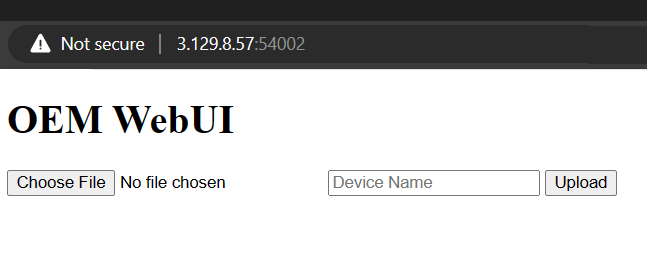
\includegraphics[width=\textwidth]{webui.png}
    \caption{webUI on server side}
\end{figure}
The developers of the firmware can then choose the updated firmware file and give it the device identification (device make/model etc) and upload the firmware. After the upload process is complete, the user interface updates like the following figure and displays the transaction status (from the blockchain: 1 stands for success and 0 stands for some kind of failure) and the IPFS content ID:
\begin{figure}[H]
    \centering
    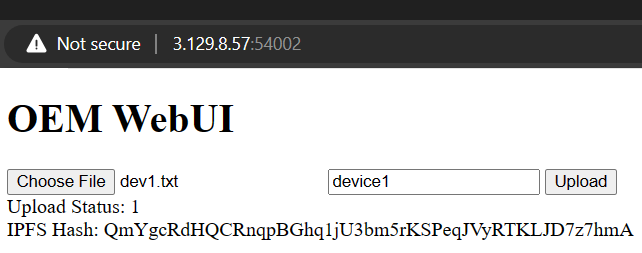
\includegraphics[width=\textwidth]{response.png}
    \caption{response after firmware is uploaded to IPFS and recorded on blockchain}
\end{figure}

On the client side, when the end user navigates to the ip address of the updater device on port 54000, the following interface is presented, and after giving the device identifier (device name or model/make etc) and pressing update button, the updater does the update process and when it is complete, presents the user with the IPFS content ID of the firmware file and the contents of the file (in utf-8 encoding) like the figure shown below:
\begin{figure}[H]
    \centering
    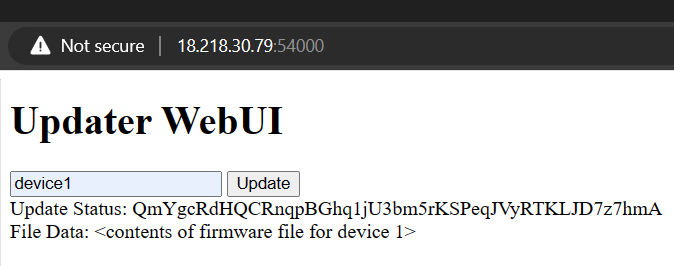
\includegraphics[width=\textwidth]{updaterResponse.png}
    \caption{response after firmware update is applied on the client side}
\end{figure}

\section{Conclusion}
This project has successfully implemented a testbed to manage firmware updates for IoT devices using blockchain and distributed storage. By integrating blockchain and distributed storage technologies, the key challenges in traditional update methods have been addressed, providing a more secure, transparent, and decentralized solution.
The design section emphasized the significance of the architecture, incorporating IPFS for decentralized storage, a Proof of Authority consensus mechanism for firmware update validation, and the use of blockchain for an immutable update history. This design ensures not only the security and reliability of firmware updates but also the scalability and efficiency of the system.
The development section showcased the implementation of the system, highlighting the utilization of Docker containers, the server-side components (Geth Signer, IPFS node, Web Server), and the client-side components (Geth Node, IPFS node, Updater). The achieved results demonstrated the successful deployment of smart contracts, mining process, and a simple and user-friendly interfaces for both server and end-user sides.
\newpage
\section{Future Work}
There are exciting avenues for future enhancements with this project:
\begin{enumerate}
    \item End-User Identity Verification: Introducing a setup phase for end-user identity verification would add an extra layer of security. Implementing a process where end-users' identities are confirmed, possibly through a Know Your Customer (KYC) procedure, would strengthen the overall system security.
    \item JWT Token Authorization: Incorporating JWT tokens for authorization can enhance security for various system endpoints. This involves issuing tokens during the setup phase, allowing authorized access to critical components such as obtaining swarm keys and enode addresses.
    \item Real-Time Firmware Update Monitoring: Developing a real-time monitoring system for firmware updates could provide administrators and end-users with immediate insights into the update process. This could include tracking the status of updates, detecting anomalies, and generating alerts in case of suspicious activities.
    \item Integration with CI/CD pipelines: A command line utility can be developed to interact with the web server on the manufacturer side so that whenever a new firmware update is made using git commits, the utility can be triggered and all the user interaction can be skipped so that those updates can be deployed to the blockchain and distributed storage automatically.
\end{enumerate}
Future work could further elevate the system's security, usability, and overall effectiveness by incorporating the above mentioned measures.
\newpage
\section{References}
\printbibliography

\end{document}
